\subsection{Pancreas}
The pancreas is commonly associated with the production of insulin and its subsequent effect on the uptake and metabolic degradation of glucose \cite{caicedo_paracrine_2013}. This function has major implications for research into disorders associated with a malfunction in the production of or response to insulin (i.e. obesity, diabetes, metabolic syndrome, etc.) and has guided much of the clinical and computational research into the structure and function of the organ \cite{woods_pancreatic_2006}. The pancreas, however, is responsible for producing a broad range of hormones and enzymes and is implicated in a considerable scope of metabolic processes. It can be thought of as an ecosystem with characteristic spatial, physiological, and environmental profiles that themselves exist in a compelling purview of phenotypes. 
\par Less frequently considered but biologically essential roles include the production of digestive enzymes, the release of neurotransmitters, and feedback regulation of major metabolic pathways. Digestive enzymes critical to peptide and saccharide breakdown include chymotrypsin, trypsin, pepsin, lipase, and pancreatic amylase and are released by acinar cells (exocrine cells of the pancreas) \cite{ianiro_digestive_2016}. The pancreas is, intuitively, the site of origin for the pancreatic duct where bicarbonate is released as a response to the presence of chyme in the duodenum \cite{hegyi_pancreatic_2011}. Further, recent research on human islets has revealed that gamma aminobutyric acid (GABA), a neurotransmitter associated with an inhibitory effect on the central and peripheral nervous systems, is released by $\beta$ cells \cite{rutter_gaba_2017}. A similar study on mouse islets has found that endocrine cells of islets express the genes implicated in the production of serotonin and respond to the presence of the neurotransmitter through a decreased insulin production \cite{chandra_neural_2009}.
\par The human pancreas sits in the posterior abdomen wall with an average weight of approximately 90 grams. It is derived from embryonic endoderm tissue and can be divided into at least four structurally distinct segments: the head, body, tail, and uncinate process \cite{g_quantification_2012} \cite{birnbaum_head_2019}.
\par Endocrine cells of the pancreas occuppy 1-2 \% of the pancreas by mass and can be divided into three types, often categorized by a characteristic secretagogue \cite{pour_are_2002}. They exist within islets (Islets of Langerhans) and can be found in clumps of between 70 to over 100 cells. $\alpha$ cells are known for secreting glucagon which is associated with low blood glucose and responsible for stimulating the release of glucose from cells, gluconeogenesis, and the breakdown of fatty acid and saccharide energy stores \cite{jiang_glucagon_2003}. $\beta$ cells are make up the highest percentage of endocrine cells within the islet and are known for producing and secreting insulin \cite{g_quantification_2012}. Insulin is often thought of as complementary to glucagon since it is associated with high blood glucose and stimulates its uptake from the blood, glycolysis, and the synthesis of fatty acid and saccharide energy stores \cite{hatting_insulin_2018}. $\delta$ cells are the least well studied and common of the major endocrine cells of the pancreas \cite{vergari_somatostatin_2020}. They secrete somatostatin, which affects cell proliferation, neurotransmission, and the release of glucagon and insulin from the aforementioned $\alpha$ and $\beta$ cells \cite{braun_somatostatin_2009}. $\epsilon$ cells comprise a very small percentage of islet cells and are responsible for the release of the hormone ghrelin, which most strongly associated with the regulation of hunger \cite{sakata_development_2019}.
\par Electrical activity in these endocrine cells is a product of the flow of various ion species across their respective electrochemical gradients \cite{riz_mathematical_2014}. These ions flow through protein channels with different gating properties (i.e. voltage-dependent, pH-dependent, substrate-dependent, etc.) and are responsible for changes in membrane potential or enzymatic cascades that facilitate communication between cells, tissues, and organs. 
\par The Zhang-Liu hypothesis outlines the biological basis of electrical excitability in $\beta$ cells and has recently been generalized to $\alpha$ and $\delta$ cells \cite{briant_functional_2017}. According to this hypothesis, electrical activity is stimulated by the intake of glucose, which after degradation through glycolysis and further processing in the Kreb's Cycle, yields an increase in cyptoplasmic adenosine triphosphate (ATP). This closes ATP-dependent potassium channels and causes an initial increase in membrane potential. The change in membrane potential, in turn, results in the opening of voltage-dependent calcium channels and the intake of calcium. This current drives a spike and the influx of calcium activates various secondary messenger pathways that lead to hormone secretion.
\subsection{Modeling Electrophysiology}
The electrical excitability of neurons has long been observed, but until the mid 20th century the mechanisms behind this behavior were poorly understood. In 1952, A.L Hodgkin and A.F. Huxley released a nobel prize winning series of papers in which they developed a mathematical model that elucidated the principles of ion channel dynamics in the giant squid axon \cite{hodgkin_effect_1949}. Modern modeling of electrically excitable membranes takes its root in these papers and often includes some combination of the following equations which constituted their mathematical model \cite{riz_mathematical_2014}.
\begin{figure}[h!]\label{circ}
	\centering
	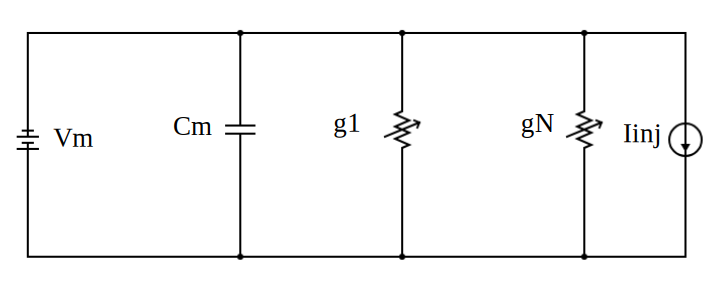
\includegraphics[scale=0.65]{Figures/circuit_labeled.png}
	\caption{Membrane as a circuit}
\end{figure}
\begin{equation}\label{hh}
\frac{dV_m}{dt} = \frac{1}{C_m} (I_{inj} - \bar{g}_k n^4 (V_m - V_k) -\bar{g}_{na} m^3 h (V_m - V_{na}) - \bar{g}_l (V_m - V_l))
\end{equation}
\begin{equation}\label{dn}
\frac{dn}{dt} = \alpha_n (V_m) (1 - n) - \beta_n (V_m) n
\end{equation}
\begin{equation}\label{dm}
\frac{dm}{dt} = \alpha_m (V_m) (1 - m) - \beta_m (V_m) m
\end{equation}
\begin{equation}\label{dh}
\frac{dh}{dt} = \alpha_h (V_m) (1 - h) - \beta_h (V_m) h
\end{equation}

\par Their first major breakthrough came in the form of an assumption; that the lipid bilayer and protein channels of the axon were analogous to capacitive and resistive elements of a circuit (see Figure 1). This circuit is subject to the same laws that would govern the flow of current if it ws to take a physical form, and thus, by Ohm's Law and Kirkoff's Second Law, equation \ref{hh} can be derived. It is worth noting that the membrane potential corresponding to an electromotive force in the equivalent circuit is determined by the various electrochemical gradients across the cell's membrane and can be quantified by a modified form of the Nernst Equation (equation \ref{Nernst}). 
\begin{equation}\label{Nernst}
E = -\frac{RT}{nF} \ln Q
\end{equation}
\par Their second major breakthrough was that ion channel permeability (represented in equation \ref{hh} as the term multiplied against the membrane potential and reversal potential: i.e. $\bar{g}_k n^4$ for the sodium channel) was dependent on membrane potential and its own state. This temporal relationship between permeability and membrane potential was represented through a series of differential equations wherein the rate of activation ($\alpha_m$) is multiplied by the proportion of closed channels and the rate of inactivation ($\beta_m$) is similarly multiplied by the proportion of open channels. These rates were modeled by the Boltzmann distribution and had to be experimentally determined.
\begin{equation}
\frac{P_o}{P_c}  = K e^{qV}
\end{equation}
\par In the above equation, the ratio of the probability of an ion channel taking an open state to the same ion channel taking a closed state is equal to the free energy difference between those states. This is determined by a modified form of Gibb's Free Energy equation ($\Delta G = -qVln(K)$). By solving for the probability of an open channel we can derive an equation similar of form to that used to represent the rate of opening of a (potassium) channel in the original Hodgkin and Huxley model (equation \ref{hhn}).
\begin{equation}
P_o = \frac{1}{1 + \frac{e^{-qV}}{K}}
\end{equation}
\begin{equation}\label{hhn}
\alpha_{n} = \frac{0.1(10-V_m)}{e^{\frac{10-V_m}{10}}-1}
\end{equation}
\subsection{Modeling Diffusion}
Many biological processes which researchers have attempted to transcribe into a computational form involve the release and uptake of various hormones across dynamic gradients (i.e. electrochemical). Often the molecules being transferred from one location to another are transformed from one state to another either by means of a reaction with a similar molecule undergoing an analogous pattern of uptake and release or by means of an enzyme in a catalytic process. Since the molecules of interest often react with each other and form an intricate system of diffusion gradients and chemical reactions, these components of computational models of such biological systems are bundled together and represented through a single system of equations known as the Kolmogorov–Petrovsky–Piskunov system (or more simply: the reaction-diffusion system) \cite{fisher_wave_1937}.
\begin{equation}\label{rxd}
\delta_t u = D \delta_x^2 u+R(u)
\end{equation}
\par In this equation, $u$ represents some macroscopic variable such as concentration or mole fraction, $D$ a diffusion coefficient, $\delta_x^2 u$ diffusion, and $R(u)$ some reaction that affects a change in $u$. This system is often used when modeling pattern formation or the equilibrium of a system involving multiple ion species \cite{kondo_reaction-diffusion_2010}. Within the context of modeling cells, reaction diffusion allows researchers to predict the path of individual ions through extracellular spaces and their general flow from one cell to another.
\subsection{Previous Models}
The development and refinement of computational models of the pancreas has been a field of interest since at least the early 1980s \cite{chay_minimal_1983}. However, much of the research in this field during this period involved investigations into the function of beta cells often without consideration of the other major endocrine cells, even excluding the effect those cells may have on beta cell function. This is understandable as the role of beta cells in the production of insulin and its association with diabetes and obesity have been long understood and observed. However, the growing body of knowledge in the field points to islets being intricate systems of endocrine cells whose form and function are best understood through their role in macro level functions of the pancreas.
\par Recently, models have refined the previous work done on islets through wider scopes of considered cells and biological processes, more rigidly determined experimental constants, and the use of more considerable hardware resources that allow for simulations with greater space and time complexity. This work will define the outline of the model developed in this thesis and includes a model of $\beta$ cells by Fridlyand and models of $\alpha$ and $\delta$ cells by Watts and Sherman \cite{fridlyand_pancreatic_2016} \cite{watts_modeling_2014}. It is worth noting that these models differ in scope, with the computational models of $\alpha$ and $\delta$ cells accounting for the production and degradation of various intermediates in metabolic pathways leading to exocytosis while the computational model of $\beta$ cells focuses only on variables directly related to changes in membrane potential.